\chapter{The Interpreter}

\textsc{Perspective}: The interpreter provides a software realization
of Icon's virtual machine. This machine is stack-based. The basic
units on which the Icon virtual machine operates are descriptors. The
instructions for the virtual machine consist of operations that
manipulate the stack, call C functions that carry out the built-in
operations of Icon, and manage the flow of control. The Icon
interpreter executes these virtual machine instructions.  It consists
of a loop in which a virtual machine instruction is fetched and
control is transferred to a section of code to perform the
corresponding operation.

\section[8.1 Stack-Based Evaluation]{8.1 Stack-Based Evaluation}

Virtual machine instructions typically push and pop data on the
interpreter stack. The interpreter stack, which is distinct from the
stack used for calls of C functions, is an array of words. The
variable \texttt{sp} points to the last word pushed on the interpreter
stack. Pushing increments \texttt{sp}, while popping decrements it. When the
interpreter executes code that corresponds to a built-in operation in
Icon, it pushes descriptors for the arguments on the interpreter stack
and calls a C function corresponding to that operation with a pointer
to the place on the interpreter stack where the arguments begin. A
null descriptor is pushed first to serve as a
{\textquotedbl}zeroth{\textquotedbl} argument (Arg0) that receives, by
convention, the result of the computation and becomes the top
descriptor on the stack when the C function returns. On a more
conventional virtual machine, the result of the computation would be
pushed on the stack, instead of being returned in an argument. The
latter method is more convenient in Icon.

To illustrate this basic mechanism, consider the expression

\iconline{ \>   ?10 }

\noindent which produces a randomly selected integer between 1 and 10,
inclusive. The corresponding virtual machine instructions are

\goodbreak
\iconcode{
\>pnull\>\>\>\>\>\>\# push null descriptor for the result\\
\>int\>\>\>10\>\>\>\# push descriptor for the integer 10\\
\>random\>\>\>\>\>\>\# compute random value
}

The instructions \texttt{pnull} and \texttt{int} operate directly on
the stack. The instruction \texttt{random} calls a C function that
computes random values.

The \texttt{pnull} instruction pushes a null descriptor:

\begin{picture}(300,100)
\put(120,32){\upetc}
\put(120,32){\dvbox{null}{n}{0}}
\put(120,32){\trboxlabel{descriptor for result (Arg0)}}
\put(120,32){\downbars}
\put(120,32){\lregptr{sp}{20}}
\end{picture}

The \texttt{int} instruction pushes a descriptor for the integer 10:

\begin{picture}(300,130)
\put(120,64){\upetc}
\put(120,64){\dvbox{null}{n}{0}}
\put(120,64){\trboxlabel{descriptor for result (Arg0)}}
\put(120,32){\dvbox{integer}{n}{10}}
\put(120,32){\trboxlabel{argument of random (Arg1)}}
\put(120,32){\downbars}
\put(120,32){\lregptr{sp}{20}}
\end{picture}

Suppose that the C function for random computes 3. It replaces the
null value of Arg0 by a descriptor for the integer 3.  When it
returns, \texttt{sp} is set to point to Arg0 and the situation is

\begin{picture}(300,100)
\put(120,32){\upetc}
\put(120,32){\dvbox{integer}{n}{3}}
\put(120,32){\downbars}
\put(120,32){\lregptr{sp}{20}}
\end{picture}

\section[8.2 Virtual Machine Instructions]{8.2 Virtual Machine Instructions}

The various aspects of expressions that appear in Icon source-language
programs are reflected, directly or indirectly, in the instruction set
for the Icon virtual machine. References to constants (literals) and
identifiers have direct correspondences in the instruction set of the
virtual machine. There is a virtual machine instruction for each
source-language operator. This is possible, since the meaning of an
operation is fixed and cannot be changed during program execution. The
meaning of a function call, however, cannot be determined until it is
evaluated, and there is a single virtual machine instruction for
function invocation. The invocation of functions is described in
detail in Chapter 10.

There are several virtual machine instructions related to control
structures and the unique aspects of expression evaluation in
Icon. These are discussed in the next two chapters. A complete list of
virtual machine instructions is given in Appendix B.

\subsection[8.2.1 Constants]{8.2.1 Constants}

Four kinds of data can be represented literally in Icon programs:
integers, strings, csets, and real numbers. The four corresponding
virtual machine instructions are

\goodbreak
\iconcode{
\>  int  \>\>\>  n \>   \>\>\>\# integer n\\
\>  str  \>\>\>  n,\> a \>\>\>\# string of length n at address a\\
\>  cset \>\>\>  a \>   \>\>\>\# cset block at address a\\
\>  real \>\>\>  a \>   \>\>\>\# real block at address a
}

The values of integer literals appear as arguments of int
instructions. In the case of strings, the two arguments give its
length and the address of its first character.

The string itself is constructed by the linker and is loaded into
memory from the icode file. For csets and real numbers, the linker
constructs blocks, which are also loaded from the icode file. These
blocks are identical in format to blocks that are constructed during
program execution.

The virtual machine instructions \texttt{str}, \texttt{cset}, and
\texttt{real} push appropriate descriptors to reference the data as it
appears in the icode. For example, the virtual machine instructions
for

\iconline{ \>?"aeiou" }

\noindent are

\goodbreak
\iconcode{
\>   pnull \\
\>   str\>\>\>5,\>a \\
\>   random
}

\noindent where \texttt{\ \ a} is the address of the string
\texttt{{\textquotedbl}aeiou{\textquotedbl}}. The \texttt{pnull}
instruction pushes a null descriptor as in the previous example:

\begin{picture}(300,100)
\put(120,32){\upetc}
\put(120,32){\dvbox{null}{n}{0}}
\put(120,32){\trboxlabel{descriptor for result (Arg0)}}
\put(120,32){\downbars}
\put(120,32){\lregptr{sp}{20}}
\end{picture}

The \texttt{str} instruction constructs a descriptor for the string
\texttt{{\textquotedbl}aeiou{\textquotedbl}}:

\begin{picture}(300,130)
\put(120,64){\upetc}
\put(120,64){\dvbox{null}{n}{0}}
\put(120,64){\trboxlabel{descriptor for result (Arg0)}}
\put(120,32){\dvboxptr{5}{}{40}{"aeiou"}}
\put(120,32){\trboxlabel{argument of random (Arg1)}}
\put(120,32){\downbars}
\put(120,32){\lregptr{sp}{20}}
\end{picture}

If \texttt{random} produces the string \texttt{"o"}, this string
replaces the null descriptor and the stack becomes

\begin{picture}(300,100)
\put(120,32){\upetc}
\put(120,32){\dvboxptr{1}{}{40}{"o"}}
\put(120,32){\downbars}
\put(120,32){\lregptr{sp}{20}}
\end{picture}

In reality, things are a bit more complicated. See Section 8.2.5.

\subsection[8.2.2 Identifiers]{8.2.2 Identifiers}

From the viewpoint of the interpreter, there are four kinds of
identifiers: global identifiers, static identifiers, local
identifiers, and arguments. The values of global and static
identifiers are in arrays of descriptors at fixed locations in
memory. The values of local identifiers and arguments, on the other
hand, are kept on the stack as part of the information associated with
a procedure call.

The values of the arguments in the call of a procedure are pushed on
the stack as the result of the evaluation of expressions prior to the
invocation of the procedure. The initial null values for local
identifiers are pushed on the stack when the procedure is called.

Consider the following procedure declaration:
\goodbreak
\iconcode{
procedure p(x,y)  \\
\>  local z, i, j \\
\>  j := 1 \\
\>  z := x \\
\>  \>...  \\
end
}

\noindent In the evaluation of a call to this procedure such as 
\iconline{ \>p(10,20) }

\goodbreak\noindent the stack is in the following state prior to the evaluation
of the first expression in p:

\begin{picture}(300,270)(0,-32)
\put(120,0){\dvbox{null}{n}{0}}
\put(120,0){\trboxlabel{value of j}}
\put(120,0){\lregptr{sp}{20}}
\put(120,0){\downbars}
\put(120,32){\dvbox{null}{n}{0}}
\put(120,32){\trboxlabel{value of i}}
\put(120,64){\dvbox{null}{n}{0}}
\put(120,64){\trboxlabel{value of z}}
\put(120,64){\tlboxlabel{locals}}
\put(120,64){\upetc}
\put(120,144){\dvbox{integer}{n}{20}}
\put(120,144){\trboxlabel{value of y}}
\put(120,144){\downetc}
\put(120,176){\dvbox{integer}{n}{10}}
\put(120,176){\trboxlabel{value of x}}
\put(120,176){\tlboxlabel{arguments}}
\put(120,176){\upetc}
\end{picture}

The portion of the stack between the arguments and local identifiers
is fixed in size and contains information that is saved when a
procedure is called. This information is described in Chapter 10.

There are four virtual machine instructions for constructing variable
descriptors:

\goodbreak
\iconcode{
\>global\>\>\> n\\
\>static\>\>\> n\\
\>arg\>\>\> n\\
\>local\>\>\> n
}

Identifiers of each kind are numbered starting at zero. Consequently,

%-% {\ttfamily\mdseries
%-% \ \ \ arg 0}
\iconline{ \>arg\>\>\> 0 }

\noindent pushes a variable descriptor for the first argument. In each
case, the descriptor that is pushed on the stack is a variable that
points to the descriptor for the value of the corresponding identifier.

Consider the expression

\iconline{ \>j := 1 }

The corresponding virtual machine instructions are

\goodbreak
\iconcode{
\>pnull\>\>\>\>\>\>\# push null descriptor for the result\\
\>local\>\>\>2\>\>\>\# push variable descriptor for j\\
\>int\>\>\>1\>\>\>\# push descriptor for the integer 1\\
\>asgn\>\>\>\>\>\>\# perform assignment
}

When these instructions are interpreted, the succession of stack states is

\begin{picture}(300,240)
\put(-4,32){
\begin{picture}(0,0)
\put(120,0){\dvbox{null}{n}{0}}
\put(120,0){\trboxlabel{value of j}}
\put(120,32){\dvbox{null}{n}{0}}
\put(120,32){\trboxlabel{value of i}}
\put(120,64){\dvbox{null}{n}{0}}
\put(120,64){\trboxlabel{value of z}}
\put(120,64){\tlboxlabel{locals}}
\put(120,64){\upetc}
\put(120,144){\dvbox{integer}{n}{20}}
\put(120,144){\trboxlabel{value of y}}
\put(120,144){\downetc}
\put(120,176){\dvbox{integer}{n}{10}}
\put(120,176){\trboxlabel{value of x}}
\put(120,176){\tlboxlabel{arguments}}
\put(120,176){\upetc}
\end{picture}
}
\put(120,0){\lregptr{sp}{20}}
\put(120,0){\dvbox{null}{n}{0}}
\put(120,0){\downbars}
\put(120,0){\trboxlabel{descriptor for result (Arg0)}}
\end{picture}

\ \ \ \ \ \ The Stack after \texttt{pnull}\vfill

 %--%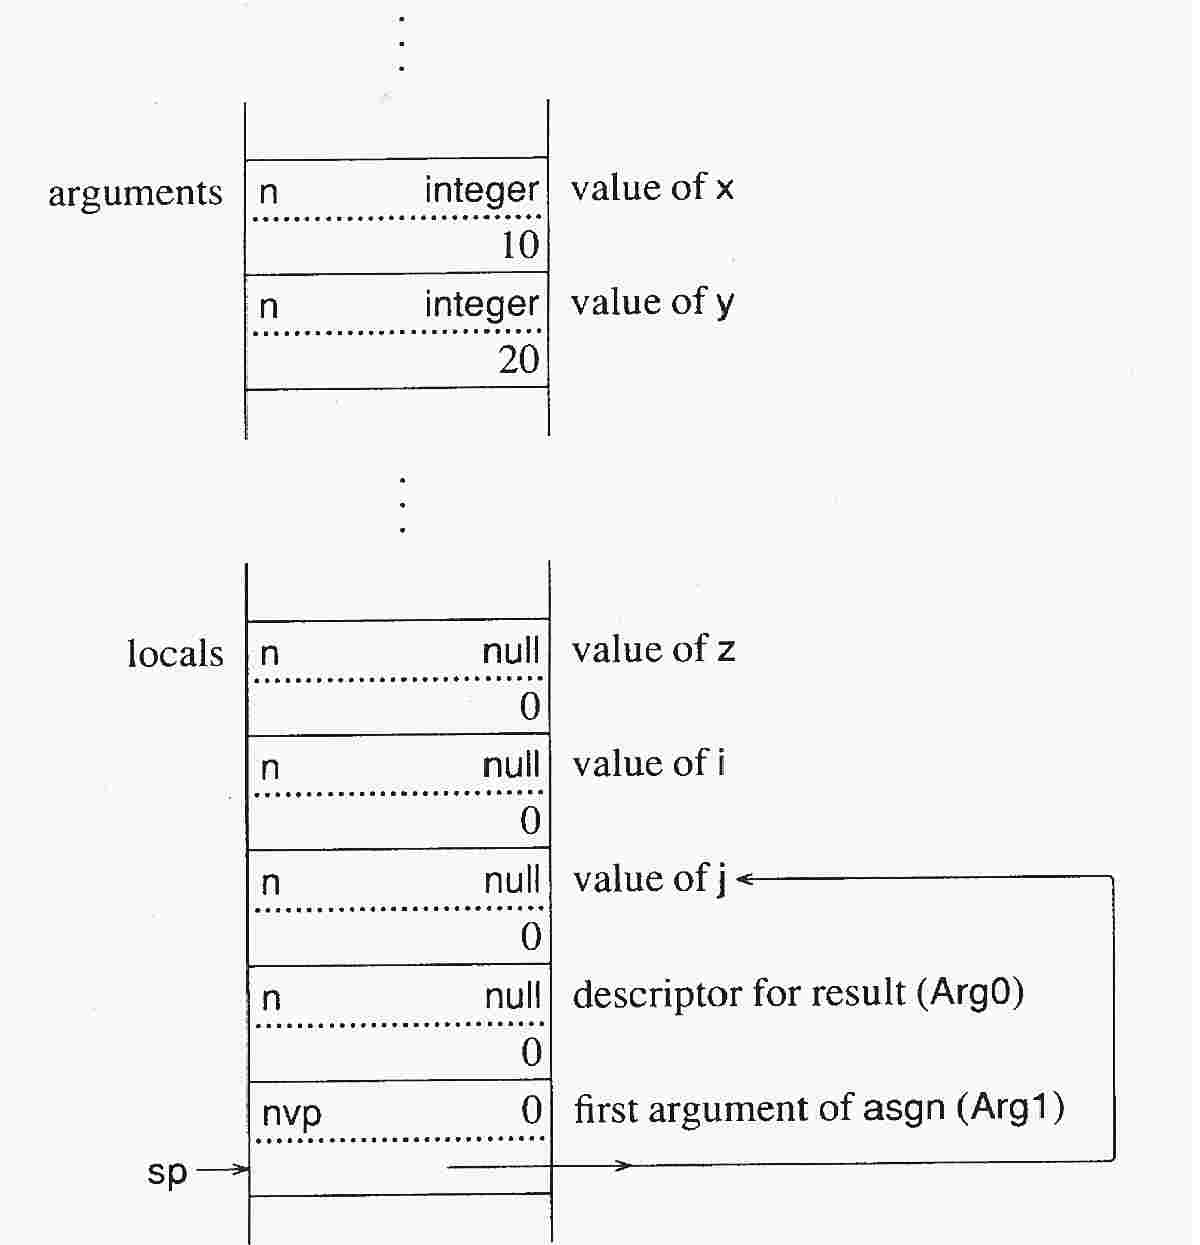
\includegraphics[width=4.0602in,height=4.1575in]{ib-img/ib-img048.jpg} 
\begin{picture}(300,310)
\put(-4,32){
\begin{picture}(300,0)
\put(-4,32){
\begin{picture}(0,0)
\put(120,0){\dvbox{null}{n}{0}}
\put(120,0){\trboxlabel{value of j}}
\put(120,32){\dvbox{null}{n}{0}}
\put(120,32){\trboxlabel{value of i}}
\put(120,64){\dvbox{null}{n}{0}}
\put(120,64){\trboxlabel{value of z}}
\put(120,64){\tlboxlabel{locals}}
\put(120,64){\upetc}
\put(120,144){\dvbox{integer}{n}{20}}
\put(120,144){\trboxlabel{value of y}}
\put(120,144){\downetc}
\put(120,176){\dvbox{integer}{n}{10}}
\put(120,176){\trboxlabel{value of x}}
\put(120,176){\tlboxlabel{arguments}}
\put(120,176){\upetc}
\end{picture}
}
\put(120,0){\dvbox{null}{n}{0}}
\put(120,0){\trboxlabel{descriptor for result (Arg0)}}
\end{picture}
}
\put(120,0){\lregptr{sp}{20}}
\put(120,0){\dvboxptr{null}{nvp}{40}{}}
\put(120,0){\downbars}
\put(120,0){\trboxlabel{first argument of asgn (Arg1)}}
\put(240,8){\line(1,0){164}}
\put(404,8){\line(0,1){80}}
\put(404,88){\vector(-1,0){120}}
\end{picture}

\ \ The Stack after \texttt{local 2}\vfill

\begin{picture}(300,380)
\put(-4,32){
\begin{picture}(0,0)
\put(-4,32){
\begin{picture}(0,0)
\put(-4,32){
\begin{picture}(0,0)
\put(120,0){\dvbox{null}{n}{0}}
\put(120,0){\trboxlabel{value of j}}
\put(120,32){\dvbox{null}{n}{0}}
\put(120,32){\trboxlabel{value of i}}
\put(120,64){\dvbox{null}{n}{0}}
\put(120,64){\trboxlabel{value of z}}
\put(120,64){\tlboxlabel{locals}}
\put(120,64){\upetc}
\put(120,144){\dvbox{integer}{n}{20}}
\put(120,144){\trboxlabel{value of y}}
\put(120,144){\downetc}
\put(120,176){\dvbox{integer}{n}{10}}
\put(120,176){\trboxlabel{value of x}}
\put(120,176){\tlboxlabel{arguments}}
\put(120,176){\upetc}
\end{picture}
}
\put(120,0){\dvbox{null}{n}{0}}
\put(120,0){\trboxlabel{descriptor for result (Arg0)}}
\end{picture}
}
\put(120,0){\dvboxptr{0}{nvp}{40}{}}
\put(120,0){\trboxlabel{first argument of asgn (Arg1)}}
\put(240,8){\line(1,0){164}}
\put(404,8){\line(0,1){80}}
\put(404,88){\vector(-1,0){120}}
\end{picture}
}
\put(120,0){\lregptr{sp}{20}}
\put(120,0){\dvbox{integer}{n}{1}}
\put(120,0){\trboxlabel{second argument of asgn (Arg2)}}
\put(120,0){\downbars}
\end{picture}

\ \ \ \ \ \ The Stack after \texttt{int 1}

\begin{picture}(300,330)(0,-30)
\put(-4,32){
\begin{picture}(300,0)
\put(120,0){\dvbox{integer}{n}{1}}
\put(120,0){\trboxlabel{value of j}}
\put(120,32){\dvbox{null}{n}{0}}
\put(120,32){\trboxlabel{value of i}}
\put(120,64){\dvbox{null}{n}{0}}
\put(120,64){\trboxlabel{value of z}}
\put(120,64){\tlboxlabel{locals}}
\put(120,64){\upetc}
\put(120,144){\dvbox{integer}{n}{20}}
\put(120,144){\trboxlabel{value of y}}
\put(120,144){\downetc}
\put(120,176){\dvbox{integer}{n}{10}}
\put(120,176){\trboxlabel{value of x}}
\put(120,176){\tlboxlabel{arguments}}
\put(120,176){\upetc}
\end{picture}
}
\put(120,0){\dvboxptr{0}{nvp}{44}}
\put(120,0){\trboxlabel{result returned by asgn}}
\put(120,0){\lregptr{sp}{20}}
\put(120,0){\downbars}
\put(240,8){\line(1,0){164}}
\put(404,8){\line(0,1){48}}
\put(404,56){\vector(-1,0){120}}
\end{picture}

\ \ \ \ The Stack after \texttt{asgn}

Note that \texttt{asgn} assigns the value of its second argument to
\texttt{j} and overwrites Arg0 with a variable descriptor, which is
left on the top of the stack.

Similarly, the virtual machine instructions for

\iconline{ \>z := x }

are

\goodbreak\iconcode{
\>pnull\\
\>local\>\>\>0\\
\>arg\>\>\>0\\
\>asgn
}

\noindent the states of the stack are


\begin{picture}(300,280)(0,-10)
\put(-4,32){
\begin{picture}(0,0)
\put(120,0){\dvbox{integer}{n}{1}}
\put(120,0){\trboxlabel{value of j}}
\put(120,32){\dvbox{null}{n}{0}}
\put(120,32){\trboxlabel{value of i}}
\put(120,64){\dvbox{null}{n}{0}}
\put(120,64){\trboxlabel{value of z}}
\put(120,64){\tlboxlabel{locals}}
\put(120,64){\upetc}
\put(120,144){\dvbox{integer}{n}{20}}
\put(120,144){\trboxlabel{value of y}}
\put(120,144){\downetc}
\put(120,176){\dvbox{integer}{n}{10}}
\put(120,176){\trboxlabel{value of x}}
\put(120,176){\tlboxlabel{arguments}}
\put(120,176){\upetc}
\end{picture}
}
\put(120,0){\dvbox{null}{n}{0}}
\put(120,0){\trboxlabel{descriptor for result (Arg0)}}
\put(120,0){\lregptr{sp}{20}}
\put(120,0){\downbars}
\end{picture}


\ \ The Stack after \texttt{pnull}


\begin{picture}(300,320)(0,-10)
\put(-4,32){
\begin{picture}(0,0)
\put(-4,32){
\begin{picture}(0,0)
\put(120,0){\dvbox{integer}{n}{1}}
\put(120,0){\trboxlabel{value of j}}
\put(120,32){\dvbox{null}{n}{0}}
\put(120,32){\trboxlabel{value of i}}
\put(120,64){\dvbox{null}{n}{0}}
\put(120,64){\trboxlabel{value of z}}
\put(120,64){\tlboxlabel{locals}}
\put(120,64){\upetc}
\put(120,144){\dvbox{integer}{n}{20}}
\put(120,144){\trboxlabel{value of y}}
\put(120,144){\downetc}
\put(120,176){\dvbox{integer}{n}{10}}
\put(120,176){\trboxlabel{value of x}}
\put(120,176){\tlboxlabel{arguments}}
\put(120,176){\upetc}
\end{picture}
}
\put(120,0){\dvbox{null}{n}{0}}
\put(120,0){\trboxlabel{descriptor for result (Arg0)}}
\end{picture}
}
\put(120,0){\dvboxptr{0}{nvp}{44}{}}
\put(120,0){\lregptr{sp}{20}}
\put(120,0){\trboxlabel{first argument of asgn (Arg1)}}
\put(244,8){\line(1,0){160}}
\put(404,8){\line(0,1){144}}
\put(404,152){\vector(-1,0){116}}
\put(120,0){\downbars}
\end{picture}

\ \ The Stack after \texttt{local 0}


\begin{picture}(300,300)(0,5)
\put(-4,32){
\begin{picture}(0,0)
\put(-4,32){
\begin{picture}(0,0)
\put(-4,32){
\begin{picture}(0,0)
\put(120,0){\dvbox{integer}{n}{1}}
\put(120,0){\trboxlabel{value of j}}
\put(120,32){\dvbox{null}{n}{0}}
\put(120,32){\trboxlabel{value of i}}
\put(120,64){\dvbox{null}{n}{0}}
\put(120,64){\trboxlabel{value of z}}
\put(120,64){\tlboxlabel{locals}}
\put(120,64){\upetc}
\put(120,144){\dvbox{integer}{n}{20}}
\put(120,144){\trboxlabel{value of y}}
\put(120,144){\downetc}
\put(120,176){\dvbox{integer}{n}{10}}
\put(120,176){\trboxlabel{value of x}}
\put(120,176){\tlboxlabel{arguments}}
\put(120,176){\upetc}
\end{picture}
}
\put(120,0){\dvbox{null}{n}{0}}
\put(120,0){\trboxlabel{descriptor for result (Arg0)}}
\put(120,0){\downbars}
\end{picture}
}
\put(120,0){\dvboxptr{0}{nvp}{44}{}}
\put(120,0){\trboxlabel{first argument of asgn (Arg1)}}
\put(244,8){\line(1,0){160}}
\put(404,8){\line(0,1){144}}
\put(404,152){\vector(-1,0){116}}
\end{picture}
}
\put(120,0){\dvboxptr{0}{nvp}{44}{}}
\put(120,0){\lregptr{sp}{20}}
\put(120,0){\trboxlabel{second argument of asgn (Arg2)}}
\put(120,0){\downbars}
\put(244,8){\line(1,0){180}}
\put(424,8){\line(0,1){288}}
\put(424,296){\vector(-1,0){136}}
\end{picture}

\ \ \ \ The Stack after \texttt{arg 0}

\begin{picture}(300,260)(0,5)
\put(-4,32){
\begin{picture}(0,0)
\put(120,0){\dvbox{integer}{n}{1}}
\put(120,0){\trboxlabel{value of j}}
\put(120,32){\dvbox{null}{n}{0}}
\put(120,32){\trboxlabel{value of i}}
\put(120,64){\dvbox{integer}{n}{10}}
\put(120,64){\trboxlabel{value of z}}
\put(120,64){\tlboxlabel{locals}}
\put(120,64){\upetc}
\put(120,144){\dvbox{integer}{n}{20}}
\put(120,144){\trboxlabel{value of y}}
\put(120,144){\downetc}
\put(120,176){\dvbox{integer}{n}{10}}
\put(120,176){\trboxlabel{value of x}}
\put(120,176){\tlboxlabel{arguments}}
\put(120,176){\upetc}
\end{picture}
}
\put(120,0){\dvboxptr{0}{nvp}{44}{}}
\put(120,0){\trboxlabel{result returned by asgn}}
\put(120,0){\lregptr{sp}{20}}
\put(120,0){\downbars}
\put(244,8){\line(1,0){160}}
\put(404,8){\line(0,1){112}}
\put(404,120){\vector(-1,0){116}}
\end{picture}

\ \ \ \ The Stack after \texttt{asgn}


\subsection[8.2.3 Operators]{8.2.3 \textbf{Operators}}

There is a virtual machine instruction for each of the forty-two
operators in Icon. The instructions random and asgn described
previously are examples. Casting Icon operators as virtual machine
instructions masks a considerable amount of complexity, since few Icon
operators are simple. For example, although x + y appears to be a
straightforward computation, it involves checking the types of x and
y, converting them to numeric types if they are not already numeric,
and terminating with an error message if this is not possible. If x
and y are numeric or convertible to numeric, addition is
performed. Even this is not simple, since the addition may be integer
or floating-point, depending on the types of the arguments. For
example, if x is an integer and y is a real number, the integer is
converted to a real number. None of these computations is evident in
the virtual machine instructions produced for this expression, which
are

%-% {\ttfamily
%-% \ \ \ pnull}
%-% 
%-% {\ttfamily
%-% \ \ \ local x}
%-% 
%-% {\ttfamily
%-% \ \ \ local y}
%-% 
%-% {\ttfamily
%-% \ \ \ plus}
\goodbreak
\iconcode{
\>pnull\\
\>local\>\>\> x\\
\>local\>\>\> y\\
\>plus
}

In the instructions given previously, the indices that are used to
access identifiers have been replaced by the names of the identifiers,
which are assumed to be local. This convention is followed in
subsequent virtual machine instructions for ease of reading.

Augmented assignment operations do not have separate virtual machine
instructions. Instead, the instruction \texttt{dup} first pushes a
null descriptor and then pushes a duplicate of the descriptor that was
previously on top of the stack.  For example, the virtual machine
instructions for

\iconline{ \>i +:= 1 }

are

\goodbreak
\iconcode{
\>pnull\\
\>local\>\>\> i\\
\>dup\\
\>int\>\>\> 1\\
\>plus\\
\>asgn
}

The stack after the execution of \texttt{local} is

\begin{picture}(300,120)(0,-20)
\put(120,0){\dvboxptr{0}{nvp}{40}{local i}}
\put(120,0){\lregptr{sp}{20}}
\put(120,0){\downbars}
\put(120,32){\dvbox{null}{n}{0}}
\put(120,32){\upetc}
\end{picture}

The execution of \texttt{dup} produces

\begin{picture}(300,180)(0,-20)
\put(-4,74){
\begin{picture}(0,0)(0,10)
\put(120,0){\dvboxptr{0}{nvp}{40}{local i}}
\put(120,32){\dvbox{null}{n}{0}}
\put(120,32){\upetc}
\end{picture}
}
\put(120,32){\dvbox{null}{n}{0}}
\put(120,0){\dvbox{0}{nvp}{}}
\put(120,0){\ruptr{30}{64}}
\put(120,0){\lregptr{sp}{20}}
\put(120,0){\downbars}
\end{picture}

The \texttt{dup} instruction simply takes the place of the
\texttt{pnull} and second \texttt{local} instructions in the virtual
machine instructions for

\iconline{ \>i := i + 1 }

which are

\goodbreak
\iconcode{
\>pnull\\
\>local\>\>\>i\\
\>pnull\\
\>local\>\>\>i\\
\>int\>\>\>1\\
\>plus\\
\>asgn
}

In this case, only a single \texttt{local} instruction is avoided. If
the variable to which the assignment is made is not just an identifier
but, instead, a more complicated construction, as in

\iconline{ \>a[j] +:= 1 }

\noindent substantial computation may be saved by duplicating the
result of the first argument expression instead of recomputing it.

\subsection[8.2.4 Functions]{8.2.4 Functions}

While the meaning of an operation is fixed and can be translated into
a specific virtual machine instruction, the meaning of a function call
can change during program execution. The value of the function also
can be computed. as in

\iconline{ \>(p[i])(x, y) }

The general form of a call is

\iconline{
\>\textit{expr0(expr1, expr2, } ..., \textit{exprn)}
}
The corresponding virtual machine instructions are

\goodbreak
\iconcode{
\>code for expr0\\
\>code for expr1\\
\>code for expr2\\
\>\>...\\
\>code for exprn\\
\>invoke n
}

The \texttt{invoke} instruction is relatively complicated, since the
value of \textit{expr0 }may be a procedure, an integer (for mutual
evaluation), or even a value that is erroneous. Function invocation is
discussed in detail in Chapter 10.

\subsection[8.2.5 Self-Modifying Instructions]{8.2.5 Self-Modifying Instructions}

Seven opcodes, including several described in the preceding
sections, contain operands whose values are addresses within the
virtual machine icode. The linker cannot know these run-time
addresses, so instead, it generates the instructions with byte
offsets, relative to the current instruction.  At runtime the
interpreter obtains the address in question by adding the current
instruction pointer to the offset.  In order to avoid repeating this
calculation every time the instruction executes, the interpreter
stores the pointer in place of the offset and modifies the opcode to
indicate that the offset has been converted to a pointer.  The self
modifying instructions and their address-holding counterparts are:

\iconcode{
\>   str    \>\>\>\> Astr \\
\>   cset   \>\>\>\> Astr\\
\>   real   \>\>\>\> Areal\\
\>   global \>\>\>\> Aglobal \\
\>   static \>\>\>\> Astatic\\
\>   goto   \>\>\>\> Agoto\\
\>   mark   \>\>\>\> Amark
}

The details of the \texttt{str} instruction illustrate the code for
self-modifying instructions. There are several points of interest. The
opcode must be modified from \texttt{Op\_Str} to \texttt{Op\_Astr} and
its offset operand modified to contain a pointer.  Depending on
whether Concurrent is enabled, the self-modification of the
instruction is done by either two "Put" macros
(\texttt{PutOp(Op\_Astr)} on the current opcode and
\texttt{PutWord(opnd)}), or by a \texttt{PutInstr(Op\_Astr, opnd, 2)}
after the instruction pointer is referring to the operand.  This is
because these self-modifying instructions create a race condition when
executed concurrently and thus require mutex locks.  After
(potentially) waiting to obtain a lock, the instruction must check
again to see if a competing thread has already modified its opcode,
and if so, it jumps down to the code for \texttt{Op\_Astr}.


\iconcode{
\>\>\>	 case Op\_Str:		/* string */ \\
\#ifdef Concurrent \\
\>\>\>\>    MUTEX\_LOCKID(MTX\_OP\_ASTR); \\
\>\>\>\>    if (ipc.op[-1] == Op\_Astr) \{ \\
\>\>\>\>\>     MUTEX\_UNLOCKID(MTX\_OP\_ASTR); goto L\_astr; \} \\
\#else					/*Concurrent*/ \\
\>\>\>\>    PutOp(Op\_Astr); \\
\#endif					/*Concurrent*/ \\
\>\>\>\>    PushVal(GetWord) \\
\ \\
\>\>\>\>	... \\
\>\>\>\>       opnd = (word)strcons + GetWord; \\
\ \\
\#ifdef Concurrent \\
\>\>\>\>    PutInstr(Op\_Astr, opnd, 2); \\
\#else					/*Concurrent*/ \\
\>\>\>\>    PutWord(opnd); \\
\#endif					/*Concurrent*/ \\
\>\>\>\>    PushAVal(opnd); \\
\>\>\>\>    InterpEVValD((dptr)(rsp-1), e\_literal); \\
\ \\
\>\>\>\>    MUTEX\_UNLOCKID(MTX\_OP\_ASTR); \\
\>\>\>\>    break; \\
\ \\
\>\>\>	 case Op\_Astr:		/* string, absolute address */ \\
L\_astr: \\
\>\>\>\>    PushVal(GetWord); \\
\>\>\>\>    PushAVal(GetWord); \\
\>\>\>\>    InterpEVValD((dptr)(rsp-1), e\_literal); \\
\>\>\>\>    break;
}


\section[8.3 The Interpreter Proper]{8.3 The Interpreter Proper}
\subsection[8.3.1 The Interpreter Loop]{8.3.1 The Interpreter Loop}

The interpreter, which is called \texttt{interp()}, is basically
simple in structure. It maintains a location in the icode
(\texttt{ipc}) and begins by fetching the instruction pointed to by
\texttt{ipc} and incrementing \texttt{ipc} to the next location. It
then branches to a section of code for processing the virtual machine
instruction that it fetched. The interpreter loop is

%-% {\ttfamily\mdseries
%-% \ \ \ for (;;) \{}
%-% 
%-% {\ttfamily\mdseries
%-% \ \ \ \ \ \ op = GetWord;}
%-% 
%-% {\ttfamily\mdseries
%-% \ \ \ \ \ \ switch (op) \{}
%-% 
%-% {\ttfamily\mdseries
%-% \ \ \ \ \ \ \ \ \ ...}
%-% 
%-% {\ttfamily\mdseries
%-% \ \ \ \ \ \ \ \ \ case Op\_Asgn:}
%-% 
%-% {\ttfamily\mdseries
%-% \ \ \ \ \ \ \ \ \ ...}
%-% 
%-% {\ttfamily\mdseries
%-% \ \ \ \ \ \ \ \ \ case Op\_Plus:}
%-% 
%-% {\ttfamily\mdseries
%-% \ \ \ \ \ \ \ \ \ ...}
%-% 
%-% {\ttfamily\mdseries
%-% \ \ \ \ \ \ \ \ \ \}}
%-% 
%-% {\ttfamily\mdseries
%-% \ \ \ \ \ \ continue;}
%-% 
%-% {\ttfamily\mdseries
%-% \ \ \ \ \ \ \ \ \ ...}
%-% 
%-% {\ttfamily\mdseries
%-% \ \ \ \ \ \ \}}
\goodbreak
\iconcode{
\>for (;;) \{\\
\>\>op = GetWord;\\
\>\>switch (op) \{\\
\>\>\>...\\
\>\>\>case Op\_Asgn:\\
\>\>\>...\\
\>\>\>case Op\_Plus:\\
\>\>\>...\\
\>\>\>\}\\
\>\>continue;\\
\>\>\>...\\
\>\>\}
}

\noindent
where \texttt{GetWord} is a macro that is defined to be \texttt{(*ipc++)}.

Macros are used extensively in the interpreter to avoid repetitious
coding and to make the interpreter easier to read.  The coding is
illustrated by the case clause for the instruction \texttt{plus}:

%-% {\ttfamily\mdseries
%-% \ \ \ case Op\_Plus:\ \ /* e1 + e2 */}
%-% 
%-% {\ttfamily\mdseries
%-% \ \ \ \ \ \ Setup\_Op(2);}
%-% 
%-% {\ttfamily\mdseries
%-% \ \ \ \ \ \ DerefArg(1);}
%-% 
%-% {\ttfamily\mdseries
%-% \ \ \ \ \ \ DerefArg(2);}
%-% 
%-% {\ttfamily\mdseries
%-% \ \ \ \ \ \ Call\_Op;}
%-% 
%-% {\ttfamily\mdseries
%-% \ \ \ \ \ \ break;}
\goodbreak
\iconcode{
\>case Op\_Plus:\ \ /* e1 + e2 */\\
\>\>Setup\_Op(2);\\
\>\>DerefArg(1);\\
\>\>DerefArg(2);\\
\>\>Call\_Op;\\
\>\>break;
}



\texttt{Setup\_Op(n)} sets up a pointer to the address of Arg0 on the
interpreter stack. The resulting code is

%-% {\ttfamily\mdseries
%-% \ \ \ rargp = (dptr)(sp - 1) - n;}
\iconline{\>rargp = (dptr)(sp - 1) - n;}

The value of \texttt{n} is the number of arguments on the stack.

\texttt{DerefArg(n)} dereferences argument \texttt{n}. If it is a
variable, it is replaced by its value. Thus, dereferencing is done in
place by changing descriptors on the interpreter stack.

\texttt{Call\_Cond} calls the appropriate C function with a pointer to
the interpreter stack as provided by \texttt{Setup\_Op(n)}. The
function itself is obtained by looking up \texttt{op} in an array of
pointers to functions.  The code produced by \texttt{Call\_Cond} is
(almost)

%-% {\ttfamily\mdseries
%-% \ \ \ (*(optab(op]) )(rargp);}
%-% 
%-% {\ttfamily\mdseries
%-% \ \ \ sp = (word * )rargp + 1:}
\goodbreak
\iconcode{
\>(*(optab(op]) )(rargp);\\
\>sp = (word * )rargp + 1:
}

In the case where a C function produces a result, as plus always does,
that result is placed in the Arg0 descriptor on the interpreter stack,
as illustrated by the examples in Chapters 4 and 5. The interpreter
adjusts sp to point to the v-word of Arg0. The break transfers control
to the end of the switch statement, where a continue statement
transfers control to the beginning of the interpreter loop, and the
next instruction is fetched.

As illustrated earlier, some virtual machine instructions have
operands, which follow the instructions in the icode. The interpreter
code for such an instruction fetches its operands. An example is

\iconline{ \>int n }

The interpreter code for int is

%-% case Op\_Int: /* integer */
%-%    PushVal(D\_Integer);
%-%    PushVal(GetWord);
%-%    break;
\goodbreak
\iconcode{
\>case Op\_Int: /* integer */\\
\>PushVal(D\_Integer);\\
\>PushVal(GetWord);\\
\>break;
}

\texttt{PushVal(x)} pushes x onto the interpreter stack. Thus, the descriptor
for the integer is constructed by first pushing the constant \texttt{D\_Integer}
for the d-word and then pushing the fetched operand for the v-word.

\subsection[8.3.2 Interpreter State Variables]{8.3.2 Interpreter State Variables}

The state of the interpreter is characterized by several variables,
called \textit{i-state variables}. Two i-state variables mentioned
previously are sp, the interpreter stack pointer, and ipc, the
interpreter ``program counter.''

The interpreter also pushes frames on the interpreter stack when
procedures are called. Such frames are analogous to the frames pushed
on the C stack when a C function is called, and contain information
(typically i-state variables) that is saved when a procedure is called
and restored when a procedure returns. There are other kinds of frames
for special aspects of expression evaluation; these are described in
Chapter 9. Pointers to frames are themselves i-state variables.

The proper maintenance of i-state variables is a central aspect of the
interpreter and is discussed in detail in the next two chapters.

Retrospective: The interpreter models, in software, the hardware of a
cpu. The instruction fetch, the execution of operations, and the flow
of control are basically the same as that in hardware execution, as is
the use of a stack.

An interpreter offers great flexibility. It is easy to add virtual
machine instructions, change existing ones, or change how they are
implemented. Tracking and monitoring also are easy to add. The
interpreter is machine-independent and portable. These advantages
outweigh the loss in efficiency associated with emulating hardware in
software.

\bigskip

\noindent\textbf{EXERCISES}

\liststyleLvi
\begin{enumerate}
\item Why is it advantageous for the first argument of str to be the
length of the string, rather than its address?

\item Show the states of the stack for the execution of the virtual
machine instructions for the following Icon expressions:

\iconcode{
\>   i := i + 1 \\
\>   l := ???j
}

\item Give an example for which

\iconline{
\> expr1 := expr1 + expr2
}

produces a different result from

\iconline{
\> expr1 +:= expr2
}

\item Describe, in general terms, what would be involved in adding a
new operator to Icon.

\item Describe, in general terms, what would be involved in adding a
new kind of literal to Icon.

\item Suppose that functions were bound at translation time instead of
being source-language values. How might the virtual machine be
modified to take advantage of such a feature?  What effect would this
have on the interpreter?

\end{enumerate}
